% Toolbar icon: material — a square swatch with diagonal section hatching
% (the classic material / cut-section symbol).
% NOTE: the committed svg-ui/material.svg was hand-authored to the same
% drawing (no LaTeX toolchain available); regenerating via `make ui` replaces
% it with the pdftocairo rendering of this source — same glyph either way.
\documentclass[tikz,border=2mm]{standalone}
\usetikzlibrary{arrows.meta,calc,shapes.geometric}
\begin{document}
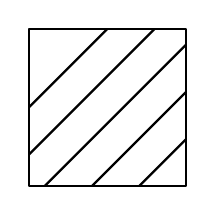
\begin{tikzpicture}[line width=1.3pt, line cap=round, line join=round, x=1mm,y=1mm]
  \draw[thick] (-10,-10) rectangle (10,10);
  % 45-degree hatching clipped to the swatch
  \begin{scope}
    \clip (-10,-10) rectangle (10,10);
    \foreach \d in {-22,-16,-10,-4,2} {
      \draw[thick] (\d,-12) -- (\d+24,12);
    }
  \end{scope}
\end{tikzpicture}
\end{document}
